%!TEX program = xelatex
% 导言区
\documentclass[12pt, letterpaper]{article}
% 文档区
\usepackage{enumerate}
\usepackage{caption}	% 可以设置脚注的各种性质
\usepackage{graphicx}	% 使用图片
\usepackage[xetex]{animate}	% 动图
\usepackage{subfigure}	% 使用子图
\usepackage{wrapfig}	% 使用嵌入的图片
\usepackage{color}	% 字体颜色
\usepackage{xcolor}
\usepackage{fullpage}	% 顾名思义
\usepackage{ctex}	% 中文支持
\usepackage{ulem}	% 字体删除线
\usepackage{amsmath}	% 公式换行
\usepackage[colorlinks,linkcolor=blue]{hyperref}	% 插入超链接
\usepackage{mathrsfs}  	% 花体
\usepackage{listings}	% 代码渲染

\lstdefinestyle{Python}{
    language        = Python,
    frame           = lines, 
    basicstyle      = \footnotesize,
    keywordstyle    = \color{blue},
    stringstyle     = \color{green},
    commentstyle    = \color{red}\ttfamily
}


\title{特征提取和特征工程。}

% 正文区
\begin{document}
% 标题
\maketitle
% 目录
\tableofcontents

\newpage
总括
本章内容不多,但是需要用到一些数学知识。尤其是一些线性代数的知识。恰好上一张的Fisher变换和MSE还没有总结,在这一章的第二节里一起总结了吧。

言归正传,前面讨论的分类器设计,都是在已经给出了特征的前提下。而这个前提想要很好的达到是不易的。因为一个合适的特征选取可以让后面的工作极大的简化,极大的影响着性能。


\section{特征提取的目的(准则)}
特征数量显然不是越多越好,甚至应该是越少越好(假如准确率能够保证的话)。一些数学方法,例如比值、指数或者对数等组合计算的应用,可能让特征的有用信息更加突出,抑制无用信息(例如取对数可以更加直观的看到大尺度下数据的变化)。特征工程也需要在保证一定分类精度的前提下,经过选择或变换处理,减少特征维数,即进行“降维”处理,使分类器实现快速、准确和高效的分类。

\begin{enumerate}
\item 去除模棱两可的、不易判别的特征
\item 所提供的数据不要重复,\textbf{即去掉那些相关性强且没有增加更多分类信息的特征。}
\end{enumerate}

\section{补充内容}
\subsection{什么是特征值、特征向量,他们的意义是什么}
\subsubsection*{特征值、特征向量的定义}

\begin{equation}
A\vec{v}=\lambda \vec{v}
\end{equation}
$v$是某一个空间下的一个向量,假如使用矩阵$A$对向量$v$进行线性变换$A\vec{v}$,变换的结果依旧在$v$所在的直线上,只是大小变为$\vec{v}$的$\lambda$倍。
\textbf{$v$称为矩阵$A$的特征值,$\vec{v}$称为特征向量。}

显然,特征向量所在直线上的向量都是特征向量:
$$
\alpha A\vec{v}=\alpha\lambda\vec{v}
$$
特征向量所在的直线(可能不止一条)包含了所有的特征向量,我们称为特征空间。
\subsubsection*{特征值分解}
\begin{enumerate}
\item 一般矩阵的特征值分解:

假如矩阵$A$是$N\times N$一个满秩方阵(换句话说,可以对角化或者有$N\times N$个特征向量),那么就可以有如下的特征值分解:
\begin{equation}
A = P\Lambda P^{-1}
\end{equation}

\item 对称矩阵的特征值分解

假如$1$中的$A$还是一个对称矩阵,就可以有:
\begin{equation}
A = P\Lambda P^T
\end{equation}
\href{https://zhidao.baidu.com/question/569597844.html}{正交矩阵的逆等于其转置。}
\end{enumerate}



\subsubsection*{运动的速度和方向}
假设二维空间中有一矩阵
$$
A = \left[
\begin{matrix}
1 &1\\
1&0\\
\end{matrix}
\right]
$$
有一个初始的点$\vec{v}=[1,1]$,对该点不断的乘矩阵$A$。即循环执行:
$\vec{v}=A.dot(\vec{v})$。最终$\vec{v}$会沿着矩阵$A$的特征值最大的特征向量方向快速增长。使用$Python$计算矩阵$A$的特征值和特征向量可得:

\begin{lstlisting}[style = Python]
from numpy import linalg as LA
import numpy as np
A = np.array([[1,1],[1,0]])
v = np.array([[1],[0]])
v = A.dot(v)
v = A.dot(v)
...
v = A.dot(v)
lbda,feature_vec = LA.eig(A)
v
lbda
feature
\end{lstlisting}
可以得到:

$$
v = \left[
\begin{matrix}
1597 \\
987
\end{matrix}
\right]
lbda = \left[
\begin{matrix}
1.61803399& -0.61803399
\end{matrix}
\right]
feature_vec = \left[
\begin{matrix}
0.85065081 & -0.52573111 \\
0.52573111 &  0.85065081
\end{matrix}
\right]
$$
显然,$\frac{1597}{987}\approx1.6 \approx \frac{0.85}{0.52}
$
特征值和矩阵的对角化有着密切的联系。
\textbf{
假如矩阵$A$可以对角化,那么就可以通过相似矩阵进行下列的特征值分解:}
\begin{equation}
A=P\Lambda P^{-1}
\end{equation}
\textbf{
其中,$P$的列向量是单位化的特征向量。$\Lambda$是对角矩阵。对角线的元素就是从大到小排列的特征值}。假如$A$是一个\textbf{对称矩阵},那么$P$的各个列向量(特征向量)相互正交。

对于方阵而言,矩阵不会进行纬度的升降,所以矩阵代表的运动实际上只有两种:
\begin{itemize}
\item 
旋转:特征向量指明了拉伸的方向
\item 
拉伸:特征值就是拉伸的大小
\end{itemize}
类比于正常的$xyz$坐标系,即可明白这是显然的。

\subsubsection*{应用}
\begin{enumerate}
\item 控制系统

上述的烧水系统是不收敛的,但是变换$A$使得$\lambda=1$,系统就是稳定的。
\item 

图片压缩。假如一个图片可以写成$512\times 512$的矩阵。那么可以进行特征值分解:
$$
A=P\Lambda P^{-1}
$$
$\Lambda$是对角阵,其对角线元素就是从大到小排列的特征值。
我们可以只保留前$50$个特征值(其他的都填$0$),输出图像就是原图像的压缩。一般来说,假如取一两百个特征向量,就能获得所有特征值之和的百分之九十了,其他的特征值就可以扔掉了。
\end{enumerate}


\subsection{PCA主成分分析法}
以下内容来自维基百科,说的非常简单明了:
\subsubsection{概括}
在多元统计分析中,主成分分析(英语:Principal components analysis,PCA)是一种\textbf{统计分析、简化数据集}的方法。
它利用\textbf{正交变换}来对一系列可能相关的变量的观测值进行线性变换,从而\textbf{投影为一系列线性不相关变量的值},这些不相关变量称为主成分(Principal Components)。

具体地,主成分可以看做一个线性方程,其包含一系列线性系数来指示投影方向。PCA对原始数据的正则化或预处理敏感(相对缩放)。
\subsubsection*{基本思想}
\begin{enumerate}
\item 将坐标轴中心移到数据的中心,然后旋转坐标轴,使得数据在C1轴上的上的方差最大,即全部n个数据个体在该方向上的投影最为分散。意味着更多的信息被保留下来。C1成为第一主成分。\textbf{这一步称为标准化}。
\item 
C2第二主成分:找一个C2,使得C2与C1的协方差(相关系数)为0,以免与C1信息重叠,并且使数据在该方向的方差尽量最大。
\item 以此类推,找到第三主成分,第四主成分。。。。第p个主成分。p个随机变量可以有p个主成分。
\end{enumerate}
\textbf{主成分分析经常用于减少数据集的维数,同时保持数据集中的对方差贡献最大的特征}。这是通过保留低阶主成分,忽略高阶主成分做到的。这样低阶成分往往能够保留住数据的最重要方面。

\subsubsection{示例说明:红酒}
假设有很多瓶红酒,对于红酒这一个对象,分析它的两个特征(例如颜色浓淡和酒精含量)。对于下图而言,这两个特征显然是相关的(无关红酒的其他特征,这俩特性就是相关)。
\begin{figure}[ht]
\centering
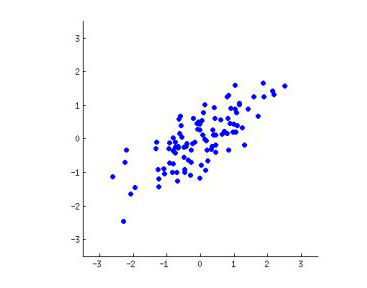
\includegraphics[scale=0.5]{两个特征.jpg}
\caption{很多瓶红酒的两个特征}
\end{figure}

首先要做的是找到“红酒云”的中心点:\textbf{两个变量的均值构成的空间中的点。}

然后以该点为轴心,画一条过该点的直线。让这条直线不断的旋转,并把所有点都投影在该直线上。

假设某个点到该直线的投影距离为$d$,投影点到中心点的距离为$m$,那么一定有$d^2+m^2$等于某一定值。该值等于原始点到中心点的距离!(勾股定理)

即整体样本的“最大方差”(红点在直线上的散布)和“最小误差”(投影距离之和,也称重建误差,)将同时达到,也就是当直线指向我在红酒云两侧标出的品红色短线时。这一直线对应于PCA将构建的新红酒属性。


\href{https://www.zhihu.com/question/41120789/answer/474222214}{动图请参考这里。}
\subsubsection{PCA与特征值和特征向量}
再次明确PCA的目标:\textbf{正交基进行降维的同时又尽量保留原始的信息。
即使得样本点$x$变换到这组正交基后使得行向量(特征)之间的协方差为0,而每个行向量的方差尽可能大。}
例如,假如有
$$
C_x = 
\left[
\begin{matrix}
C_{11} & C_{12}& \ldots&C_{1n}\\
C_{21} & C_{22}& \ldots&C_{2n}\\
\vdots& \vdots&\ddots&\vdots \\
C_{n1}& C_{n2}&\ldots&C_{nn}\\
\end{matrix}
\right]
$$
我们使用一种变换$Y=Qx$,使得变换之后的$Y$的协方差矩阵是对角矩阵(这是一定的,因为$conv(\mathbf{x},\mathbf{y})=conv(\mathbf{x},\mathbf{y})$),即$Y$中的各个变量尽可能的不相关。

对于原始数据的协方差矩阵$C_x=\frac{1}{n}xx^T$是一个对称矩阵(注意,其中$x$已经进行了去中心化$x=x-\mu$)。对于一个对阵矩阵,我们总可以对其有如下变换:
\begin{equation}
C_x = P\Lambda P^T
\end{equation}
如上文所述,$P$是一个列向量为特征向量且相互正交的矩阵。\textbf{而$\Lambda$就是一个对角矩阵。}

对于变换后的数据$Y=Qx$,其方差为$C_y=\frac{1}{n}yy^T$:
\begin{equation}
C_y=\frac{1}{n}Qxx^TQ^T=Q(\frac{1}{n}xx^T)Q^T=QC_xQ^T
\end{equation}
$PCA$的最终期望就是要是的$C_y$是一个对角矩阵。

\textbf{对$(5)$式进行变换},可以得到:
\begin{equation}
\Lambda = P^TC_xP
\end{equation}
可以进行这样的变换的一个定理是正交矩阵($P$)的转置等于其逆矩阵。
显然$\Lambda$就是要求的$C_y$,此时的$Q$有:
\begin{equation}
Q=P^T
\end{equation}

\href{https://seanlee97.github.io/2018/03/29/从特征值特征向量去理解PCA/}{参考}
\subsubsection*{什么是主成分?如何降维?}
有了$(8)$式,$Y=Qx$,其中$Q=P^T$。当想降低维度的时候,可以选取特征值所代表的特征向量作为$P$。以此来实现降维。具体的例子可以参考上文的参考。
参考:
\begin{itemize}
\item 
\href{https://blog.csdn.net/OldMonkeyYu_s/article/details/45766543}{PCA和K-L变换}
\item 
\href{https://blog.csdn.net/animaldww/article/details/5642923}{协方差矩阵和相关矩阵}
\item R.D课本 P94页,从代价函数的角度和讲述PCA算法,以及为什么要选取最大的特征值对应的特征向量最为主成分。
\end{itemize}

\subsection{K-L变换及其和PCA之间的关系}
PCA研究的是协方差矩阵,而K-L变换研究的是原始样本数据的相关矩阵。
\underline{而标准化的样本数据的协方差矩阵就是原始样本数据的相关矩阵}。
这里的标准化是指:正态化,即将原始数据处理成均值为0,方差为1的标准数据。


\subsection{Fisher变换}
\subsubsection*{理清PCA和Fisher算法的区别}
首先要说明的是,PCA算法是一种特征提取的算法。例如,假设现在要进行红酒品类的辨别,红酒本身有许多的特性。这些特性是每一种红酒都有的。但是特性过多,我们期望减少特征。可以使用PCA算法找到表示多种特征的最佳方法。从而实现降低特征空间的维度。

而Fisher判别是一种通过降低维度来分类的方法。在高纬空间中往往无法使用一种线性函数来分类,而使用非线性函数分类的设计成本太高。但是通过降低维度,却能够更好的实现分类。但到底能不能通过降维实现又快又简单又好的分类,只能通过尝试。

总体上说,PCA算法对于代表数据样本,从而实现降低特征空间的维度很有效,但并没有理由表明降低维度时选取的主成分对区分不同的类别有什么大作用。Fisher的目的是把数据映射到低维空间,从而进行分类的一种算法。

PCA和Fisher算法虽然在思想上有些相似,但是其目的和本质是完全不同的,PCA是特征工程中的算法,而Fisher是一种分类器算法。

\subsubsection*{Fisher算法的目的和依据}
Fisher算法最终想要达到的目的,是使得降低维度之后的不同种类的数据\textbf{尽可能的分得开。}降低维度的方法是映射,即通过变换:
$$
y= \mathbf{w^Tx}
$$
实现。假如$||w||=1$,那么$y$就是把$x$往方向为$w$的直线进行投影的结果。后面将会看到$w$的幅值并不重要,其方向更加重要。

Fisher判别的任务就是在讨论找到最佳的直线方向$w$,以达到最好的分类效果。


假设有两类,分别为$m_1,m_2$,两类的均值向量为:
$$\mathbf{m}_i=\frac{1}{n_i}\sum_{\mathbf{x}\in \mathscr{D}_i}\mathbf{x}$$
$n_i$代表第$i$类的样本总数,$\mathbf{x}\in \mathscr{D}_i$代表第$i$类内的样本点。
那么投影之后的样本均值就是:
$$
\begin{aligned}
\bar{m_i}&=\frac{1}{n_i}\sum_{y\in \mathscr{Y}_i}y\\
&=\frac{1}{n_i}\sum_{\mathbf{x}\in \mathscr{D}_i}\mathbf{w^Tx}=\mathbf{w^Tm_i}
\end{aligned}
$$
也就恰好是原样本均值$\mathbf{m_i}$的投影。

那么很直接的,投影之后的样本均值差就是:
$$
|\bar{m_1}-\bar{m_2}|=|\mathbf{w^T}(\mathbf{m}_1-\mathbf{m}_2)|
$$
投影之后的类别$i$内的类内散布就可以写为:
$$
\bar{s_i}^2=\sum_{y\in \mathscr{Y}_i}(y-\bar{m_i}^2)
$$
这样的话,$\frac{1}{n}(\bar{s_1}^2+\bar{s_2}^2)$就是全部数据的总体的方差的估计。(另外需要提一遍:\textbf{
类内散度矩阵=类内离散度矩阵=类内离差阵=协方差矩阵×(n-1)})
即投影之后的均值差等于投影之前的均值差的投影。(有点绕,但是这是很显然的)。

看起来好像增加$\mathbf{w}$就可以得到任意大小的投影样本均值之差,从而实现更加易分离的数据。但投影样本之差的大小总是相对的,否则问题就失去了意义。例如,就算增大了均值之差,类内的样本点的离散程度也会随之变化,并不会导致数据更加可分。这点也是显而易见的(想像成成比例拉伸坐标轴)。

能不能分辨两个类主要看两方面:一是两个类别的中心是否离得够远。二是看两个类别的数据分布是否足够集中。根据这两个原则,设计出了下面的准则函数:
\begin{equation}
\mathbf{J(w)}=\frac{|\bar{m_1}-\bar{m_2}|^2}{\bar{s_1}^2+\bar{s_2}^2}
\label{a}
\end{equation}

我们需要把$\mathbf{J(w)}$写成关于$\mathbf{w}$的表达式。
把$y,\mathbf{x},\mathbf{m_i}$的关系带入到$s_i$中可以得到:
$$
\begin{aligned}
\bar{s_i}^2&=\sum_{\mathbf{x\in \mathscr{D}_i}}(\mathbf{w^Tx}-\mathbf{w^Tm_i})^2\\
&=\sum_{\mathbf{x\in \mathscr{D}_i}}(\mathbf{w^Tx}-\mathbf{w^Tm_i})(\mathbf{w^Tx}-\mathbf{w^Tm_i})^T\\
&=\sum_{\mathbf{x\in \mathscr{D}_i}}\mathbf{w^T}(\mathbf{x}-\mathbf{m_i})(\mathbf{x}-\mathbf{m_i})^T\mathbf{w}\\
&=\mathbf{w^T}\mathbf{S}_i\mathbf{w}
\end{aligned}
$$
其中,
$$
\mathbf{S_i}=\sum_{\mathbf{x\in \mathscr{D}_i}}(\mathbf{x}-\mathbf{m_i})(\mathbf{x}-\mathbf{m_i})^T
$$
是原特征空间下的$i$类的类内散布矩阵。显然散布矩阵的变换就不像均值向量以及均值向量差的变换那么简单了。

可以定义总的散布矩阵是:
$$
\mathbf{S}_W=\mathbf{S}_1 + \mathbf{S}_2
$$
根据(\ref{a}),其分母可以变成:
$$ 
\bar{s_1}^2 + \bar{s_2}^2 = \mathbf{w^TS_ww}
$$

同理,此时的分子为:
$$
\begin{aligned}
(\bar{m_1}-\bar{m_2})^2&=(\mathbf{w^Tm_1}-\mathbf{w^Tm_2})^2\\
&=(\mathbf{w^Tm_1}-\mathbf{w^Tm_2})(\mathbf{w^Tm_1}-\mathbf{w^Tm_2})^T\\
&=\mathbf{w^T}(\mathbf{m_1}-\mathbf{m_2})(\mathbf{m_1}-\mathbf{m_2})^T\mathbf{w}\\
&=\mathbf{w^T}\mathbf{S_B}\mathbf{w}
\end{aligned}
$$
其中,
$$
\mathbf{S_B}=(\mathbf{m_1}-\mathbf{m_2})(\mathbf{m_1}-\mathbf{m_2})^T
$$
称为总类间散布矩阵。上述的总类内散布矩阵和总类间散布矩阵都是对称且半正定的矩阵。

所以此时的准则函数可以写成:
\begin{equation}
\mathbf{J(w)}=\frac{\mathbf{w^TS_Bw}}{\mathbf{w^TS_ww}}
\end{equation}
目的是:求解使得$\mathbf{J(\cdot)}$最大化的$\mathbf{w}$。求解过程详见R.D课本P98页。求解结果为:
$$
\mathbf{w}=\mathbf{S_w}^{-1}(\mathbf{m_1}-\mathbf{m_2})
$$

这样,我们就得到了Fisher可分性判据下的$\mathbf{w}$,这个$\mathbf{w}$就是使得类间散布和类内散布的比值(也就是(\ref{a})代表的含义)达到最大的线性函数。
这个向量$\mathbf{w}$又是也被称作“典范向量”。这样,\textbf{问题就从一个d维问题转化成了一个更容易分析和处理的一维问题。}

现在映射完成了,剩下的工作就是找到再一维空间中把两类分开的那个店的位置。此处要借鉴一些第二章——Bayes决策论的知识,尤其是求解判别面那一部分。

判别点方程可以设定为:
\begin{equation}
\mathbf{w^Tx}+w_0=0
\end{equation}
其中,$\mathbf{w}$按照上文的讨论可以写为:$\mathbf{w}=\Sigma^{-1}(\mathbf{\mu}_1-\mathbf{\mu}_2)$。$\mu$是样本均值,$\Sigma$是样本协方差。$w_0$是一个与$\mathbf{w}$和先验概率有关的常数。具体的判别方法请参考第二章以及课件。


\subsection{MSE最小均方误差算法及其和Fisher变换以及Bayes判别之间的关系}
\subsection{信息熵、互信息、交叉熵、K-L散度}
\subsection{奇异值分解、矩阵的张量}

\section{特征选择和特征提取的定义}
\subsubsection*{特征选择}
假设原始数据的特征空间为$n$维,即样本$x$为$(x_1,x_2,\ldots,x_n)^T$的$n$维列向量。按照某一准则选出共分类使用的子集,作为降维后的分类特征。当然,降维后的维度$m$要小于$n$。
\subsubsection*{特征提取}
显然,特征选择是依照一定的方法,删掉某些特征。但是做法往往并不十分理想,因为一般来说,原来的n个数据各自在不同程度上反映了识别对象的某些特征,\textbf{简单地删去某些特征可能会丢失较多的有用信息。}

另一种思想和特征选择相反,他不是去掉某些特征。而是利用已有的特征进行线性组合,从而\textbf{生成新的特征}:

如果将原来的特征做正交变换,\textbf{获得的每个数据都是原来n个数据的线性组合},然后从新的数据中选出少数几个,使其尽可能多地反映各类模式之间的差异,\textbf{而这些特征间又尽可能相互独立},则比单纯的选择方法更灵活、更有效。

K-L变换就是一种适用于任意概率密度函数的正交变换。



\section{特征选择}



\subsection{选取特征的不同准则}
设有n个可用作分类的测量值,为了在不降低(或尽量不降低)分类精度的前提下,减小特征空间的维数以减少计算量,需从中直接选出m个作为分类的特征。(特征选择的目的)

问题:在n个测量值中选出哪一些作为分类特征,使其具有最小的分类错误?
\begin{enumerate}
\item 一种“穷举”办法:对每种选法都用训练样本试分类一下,测出其正确分类率。显然这种办法有组合个选法,非常不可行。
\item 需寻找一种简便的可分性准则,间接判断每一种子集的优劣。
\begin{itemize}
\item 对于独立特征的选择准则
\item 一般特征的散布矩阵准则
\end{itemize}
\end{enumerate}



\subsection{对于独立特征的选择准则}
对于独立特征的选择准则
类别可分性准则应具有这样的特点,即不同类别模式特征的均值向量之间的距离应最大,而属于同一类的模式特征,其方差之和应最小。
假设各原始特征测量值是统计独立的,此时,只需对训练样本的$n$个测量值独立地进行分析,从中选出$m$个最好的作为分类特征即可。
例:对于$w_i$和$w_j$两类训练样本的特征选择

选择准则应该具有这样的特点:在这个特征维度上,不同类别模式特征的均值之间的距离应该最大,而属于同一类别的模式特征的方差应该尽可能的小(这样可以保证不同类别模式特征聚集得尽量的远)。

假设各个特征分量都是独立的,情况就比较简单了:对每一个类别的$n$个特征进行独立分析,从中选择最好的$m$个特征。

例如:对于两类分类的情况。对于第$k$维的特征,可以进行如下计算:
\begin{equation}
G_k=\frac{(m_{ik}-m_{jk})^2}{\sigma_{ik}^2+\sigma_{jk}^2},\qquad k=1,2,\ldots,n
\end{equation}
其中$m_{ik}\ m_{jk}$是第$i$和第$j$两类在第$k$维的特征的均值,$\sigma_{ik}^2\ \sigma_{jk}^2$是第$i$和第$j$两类在第$k$维的特征的方差。这是分类方式之一,但是当分布不是正态分布,这个标准可能会有问题。例如下图$(c)$。

$G_k$为正值,越大表示测度值的第$k$的分量对$w_i$和$w_j$两类的分类越有效。将${G_k,k=1,2,\ldots,n}$按大小排队,选出最大的$m$个对应的维度(也称为测度值)作为分类特征,即达到特征选择的目的。

上述方程的说明:分子越大,说明这两类在这个维度上的距离越远。分母越小,说明这两个类的总方差最大,一般来说就会导致每一类更加集中于自己的位置,更好分类。

\subsubsection*{三种不同模式分布的情况}
\begin{enumerate}[(a)]	% 罗马数字
\item 特征$x_k$的分布有很好的可分性,通过它足以分离$w_i$和$w_j$两种类别;
\item 特征分布有很大的重叠,单靠$x_k$达不到较好的分类,需要增加其它特征;
\item $w_i$类特征$x_k$的分布有两个最大值,虽然它与$w_j$的分布没有重叠,但计算$G_k$约等于$0$,此时再利用$G_k$作为可分性准则已不合适。(两个峰值的均值等于另一个类的峰值,导致分子为0)
\end{enumerate}
\begin{figure}[ht]
\centering
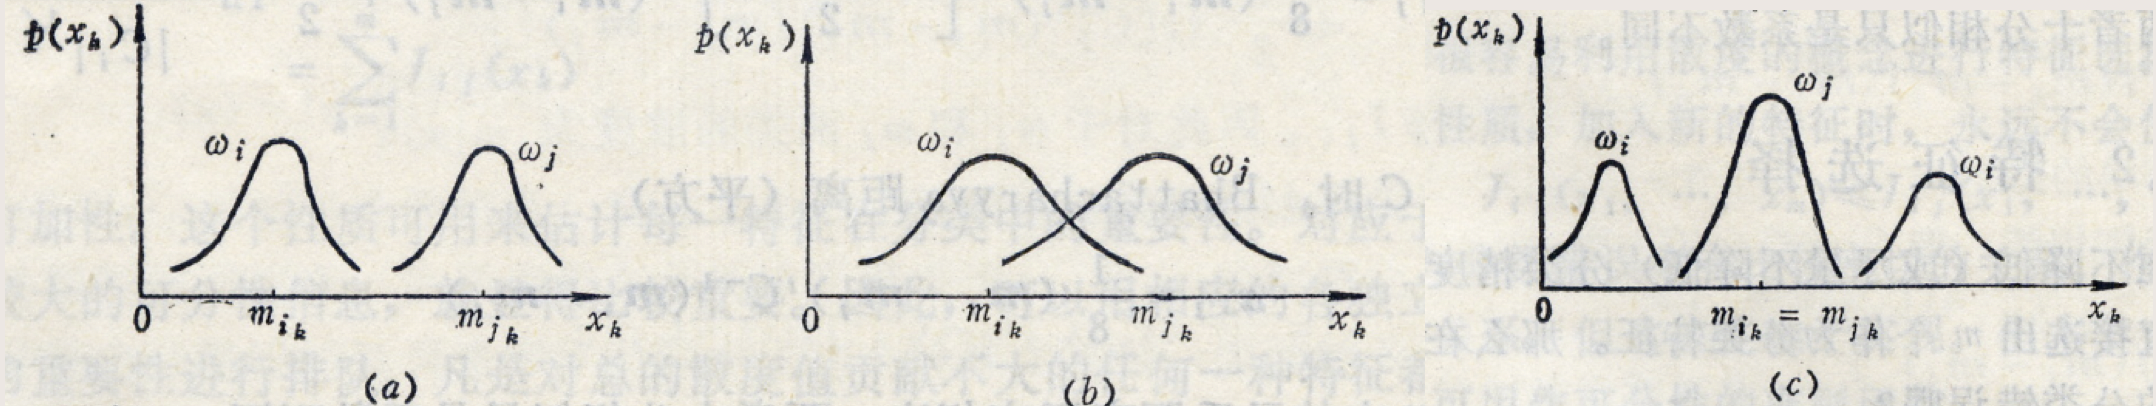
\includegraphics[scale=0.4]{三种情况.png}
\end{figure}
\subsubsection*{结论}
$(a),(b)$可以用公式分析,但是$(c)$情况下,其类概率密度函数不是或不近似正态分布,均值和方差就不足以用来估计类别的可分性,此时该准则函数不完全适用。



\subsection{模式可分的测度:均值和离散程度}
样本点的形式可以表述为$x=(x_1,x_2,\ldots,x_n)^T$。$n$为特征维度。类别$i$的样本点可以总括为$\{a^{(i)}\}$。

点和点之间的距离可以表述为两点之间的欧式距离
$$D(a,b)=||a-b||=\sqrt{(a-b)^T(a-b)}$$

点到类别的距离可以写为点到该类别内所有点的距离的均方和:
$$\overline{D^2(x,\{a^(i)\})}=\frac{1}{K}\sum_{i=1}^KD^2(x,a^{(i)})$$
其中$x$和$a^{(i)}$都是$k$维的点。
类内矩阵为

\subsubsection*{类内距离和类内散布矩阵}
\textbf{类内距离:指类内所有点到类内其他所有点的距离的均值的均值。}
$$
\overline{D^2(a^{(i)},a^{(j)})}=\frac{1}{K}\sum_{j=1}^{K}\left[\frac{1}{K-1}\sum_{i=1,i\neq j}^{K}D^2(a^{(i)},b^{(j)})\right]
$$
可以证明的是,类间距离等于不同维度上的方差和的两倍(有$n$个特征维度)。即:
$$
\overline{D^2}=2\sum_{k=1}^n\sigma_k^2
$$
其中$\sigma_k^2$为$\{a^{(i)}\}$在第$k$个分量上的无偏方差,即:
$$
\sigma_k^2=\frac{1}{K-1}\sum_{i=1}^K(a_k^{(i)}-\overline{a_k})^2
$$
{$\bar{a_k}$}是第$k$个分量方向上的均值,$a_k^{(i)}$指第$i$个采样点的第$k$个特征维度上的值。$K$代表样本点个数,$k$代表第$k$个维度。


\textbf{类内散布矩阵:各样本点围绕其均值周围的散布情况。}
另外需要提一点事实:\textbf{
类内散度矩阵=类内离散度矩阵=类内离差阵=协方差矩阵×(n-1)}
$$
S=\sum_{i=1}^K\{(a^{(i)}-m)(a^{(i)}-m)^T\}
$$
$m$是均值向量,是一个$n$维度向量$m=\frac{1}{K}\sum_{i=1}^Ka^{(i)}=(m_1,m_2,\ldots,m_n)$

\href{https://blog.csdn.net/Hearthougan/article/details/77859173}{乘n-1是因为无偏估计。}

\subsubsection*{类间距离和类间散布矩阵}
\textbf{类间距离:为简化起见,常用两类样本各自质心间的距离作为类间距离},并假设两类样本出现的概率相等,则:
$$
D^2=\sum_{k=1}^n(m_{1k}-m_{2k})^2
$$
$m_1$和$m_2$分别为两类模式的均值向量。

\textbf{类间散布矩阵可以写为:}
$$
S_{b2}=(m_1-m_2)(m_1-m_2)^T
$$

\textbf{对于c类之间的类间散布矩阵:}
$$
S_{b}=\sum_{i=1}^cP(w_i)(m_i-m_0)(m_i-m_0)^T
$$

\textbf{多类模式集散布矩阵:}
略。和Fisher一起整理。gi

其中$m_0$是多模式分布的总体均值向量。即
$$
m_0=E(x)=\sum_{i=1}^cP(w_i)m_i
$$




\subsection{一般特征的散布矩阵准则}
对于不统计独立的特征们,例如有一对特征$(x_1,x_2)$可以用这两个特征分析类间离散度、类内离散度。
\subsubsection*{散布矩阵准则}
类内散布矩阵:
$$
S_w=\sum_{i=1}^{c}P(w_i)E{(x-m_i)(x-m_i)^T|w_i}
$$
类间散布矩阵:
\begin{equation}
S_b=\sum_{i=1}^cP(w_i)(m_i-m_0)(m_i-m_0)^T
\end{equation}

直观上,类间离散度越大且类内离散度越小,则可分性越好。因此,可推导出散布矩阵准则采用如下形式:

行列式形式:$J_1=det(S_w^{-1}S_b)=\prod_i\lambda_i$

迹形式:$J_2=tr(S_w^{-1}S_b)=\sum_i\lambda_i$

\subsubsection*{限制}
这里计算的散布矩阵不受模式分布形式的限制,但需要有足够数量的模式样本才能获得有效的结果。

\section{特征提取——离散K-L变换}
详情见上述PCA。

\end{document}